%%%%%%%%%%%%%%%%%%%%%%%%%%%%%%%%%%%%%%%%%
% Beamer Presentation
% LaTeX Template
% Version 1.0 (10/11/12)
%
% This template has been downloaded from:
% http://www.LaTeXTemplates.com
%
% License:
% CC BY-NC-SA 3.0 (http://creativecommons.org/licenses/by-nc-sa/3.0/)
%
%%%%%%%%%%%%%%%%%%%%%%%%%%%%%%%%%%%%%%%%%

%----------------------------------------------------------------------------------------
%	PACKAGES AND THEMES
%----------------------------------------------------------------------------------------

\documentclass{beamer}

\mode<presentation> {

% The Beamer class comes with a number of default slide themes
% which change the colors and layouts of slides. Below this is a list
% of all the themes, uncomment each in turn to see what they look like.

%\usetheme{default}
%\usetheme{AnnArbor}
%\usetheme{Antibes}
%\usetheme{Bergen}
%\usetheme{Berkeley}
%\usetheme{Berlin}
%\usetheme{Boadilla}
%\usetheme{CambridgeUS}
%\usetheme{Copenhagen}
%\usetheme{Darmstadt}
%\usetheme{Dresden}
%\usetheme{Frankfurt}
%\usetheme{Goettingen}
%\usetheme{Hannover}
%\usetheme{Ilmenau}
%\usetheme{JuanLesPins}
\usetheme{Luebeck}
%\usetheme{Madrid}
%\usetheme{Malmoe}
%\usetheme{Marburg}
%\usetheme{Montpellier}
%\usetheme{PaloAlto}
%\usetheme{Pittsburgh}
%\usetheme{Rochester} %% Talvez - Colocar logo utfpr
%\usetheme{Singapore} %% Interessante
%\usetheme{Szeged}
%\usetheme{Warsaw}

% As well as themes, the Beamer class has a number of color themes
% for any slide theme. Uncomment each of these in turn to see how it
% changes the colors of your current slide theme.

%\usecolortheme{albatross}
%\usecolortheme{beaver}
%\usecolortheme{beetle}
\usecolortheme{crane}
%\usecolortheme{dolphin}
%\usecolortheme{dove}
%\usecolortheme{fly}
%\usecolortheme{lily}
%\usecolortheme{orchid}
%\usecolortheme{rose}
%\usecolortheme{seagull}
%\usecolortheme{seahorse}
%\usecolortheme{whale}
%\usecolortheme{wolverine}

%\setbeamertemplate{footline} % To remove the footer line in all slides uncomment this line
%\setbeamertemplate{footline}[page number] % To replace the footer line in all slides with a simple slide count uncomment this line

%\setbeamertemplate{navigation symbols}{} % To remove the navigation symbols from the bottom of all slides uncomment this line
}

\setbeamertemplate{caption}[numbered] %% Numbered figures on the project
\setbeamertemplate{headline}{} % Remove header from the title
\usepackage{float,graphicx} % Allows including images
\usepackage{booktabs} % Allows the use of \toprule, \midrule and \bottomrule in tables
\usepackage{caption}
\usepackage{hyperref}
\usepackage[brazil]{babel}
\usepackage[utf8]{inputenc}
\usepackage{subcaption}
%\usepackage{subfig}

%----------------------------------------------------------------------------------------
%	TITLE PAGE
%----------------------------------------------------------------------------------------

\title{Estágio Curricular Obrigatório} % The short title appears at the bottom of every slide, the full title is only on the title page

\author{\bf Willian Americano Lopes} % Your name
%\small walopes23@gmail.com
\institute[UTFPR] % Your institution as it will appear on the bottom of every slide, may be shorthand to save space
{
Universidade Tecnológica Federal do Paraná - Câmpus Pato Branco\\ % Your institution for the title page
DAINF - Departamento Acadêmico de Informática
\newline

%% NOVO %%
\medskip
Orientador(a): Professora Beatriz Terezinha Borsoi\newline

\medskip
walopes23@gmail.com\\
beatriz@utfpr.edu.br
}


\small \date{\today} % Date, can be changed to a custom date
%\tiny \date{05 de dezembro de 2017} % Date, can be changed to a custom date

\titlegraphic{}

\begin{document}

%%%%%%%%%%%%%%%%%%%%%%%%%%% LOGO UTFPR  
{
\setbeamertemplate{background}{%
  \raisebox{-0.65cm}{%
    \parbox[c]{3.5cm}{\centering%
      
\includegraphics[width=2cm]{Figuras/utf.pdf}%
    }%
    \parbox[c]{\dimexpr\paperwidth-5.2cm\relax}{\centering%
      {\large Universidade Tecnológica Federal do Paraná}%
    }%
  }%
}    
%%%%%%%%%%%%%%%%%%%%%%%%%%%%%%%%%%%%%%%%

%%%%%%%%%%%%%%%%%%%%%%%%%%%%%%%%%%%% PAGE NUMBER
 \addtobeamertemplate{navigation symbols}{}{%
    \usebeamerfont{footline}%
    \usebeamercolor[fg]{footline}%
    \hspace{1em}%
    \insertframenumber/\inserttotalframenumber
}
%%%%%%%%%%%%%%%%%%%%%%%%%%%%%%%%%%%%%%%%%



\begin{frame}[label=firstframe]
\titlepage % Print the title page as the first slide
\end{frame}

\begin{frame}

\frametitle{Sumário} % Table of contents slide, comment this block out to remove it
\tableofcontents % Throughout your presentation, if you choose to use \section{} and \subsection{} commands, these will automatically be printed on this slide as an overview of your presentation

\end{frame}

%----------------------------------------------------------------------------------------
%	PRESENTATION SLIDES
%----------------------------------------------------------------------------------------
%%%%%%%%%%%%%%%%%%%%%%%%%%%%%%%%%%%%%%%%%%%%%%%%%%%%%%%%%%%%%%%%%%%
%%%%%%%%%%%%%%%%%%%%%%%%%%%%%%%%%%%%%%%%%%%%%%%%%%%%%%%%%%%%%%%%%%%
\section{Introdução} % Sections can be created in order to organize your presentation into discrete blocks, all sections and subsections are automatically printed in the table of contents as an overview of the talk

%%%%%%%%%%%%%%%%%%%%%%%%%%%%%%%%%%%%%%%%%%%%%%%%%%%%%%%%%%%%%%%%%%%
\subsection{Agricultura de precisão}



%%%%%%%%%%%%%%%%%%%%%%%%%%%%%%%%%%%%%%%%%%%%%%%%%%%%%%%%%%%%%%%%%%%
\subsection{GPS}



%%%%%%%%%%%%%%%%%%%%%%%%%%%%%%%%%%%%%%%%%%%%%%%%%%%%%%%%%%%%%%%%%%%
\subsection{Microcontrolador}







%%%%%%%%%%%%%%%%%%%%%%%%%%%%%%%%%%%%%%%%%%%%%%%%%%%%%%%%%%%%%%%%%%%%%%%%%%%%%%%%%
%%%%%%%%%%%%%%%%%%%%%%%%%%%%%%%%%%%%%%%%%%%%%%%%%%%%%%%%%%%%%%%%%%%%%%%%%%%%%%%%

\section{Plano de estágio}

\subsection{A Empresa}

\begin{frame}%[noframenumbering]
\frametitle{A empresa}
\begin{columns}

	\column{0.7\linewidth}
	\begin{figure}[]
	 \centering
	 \captionsetup{width=\textwidth,font=footnotesize,textfont=bf}
	 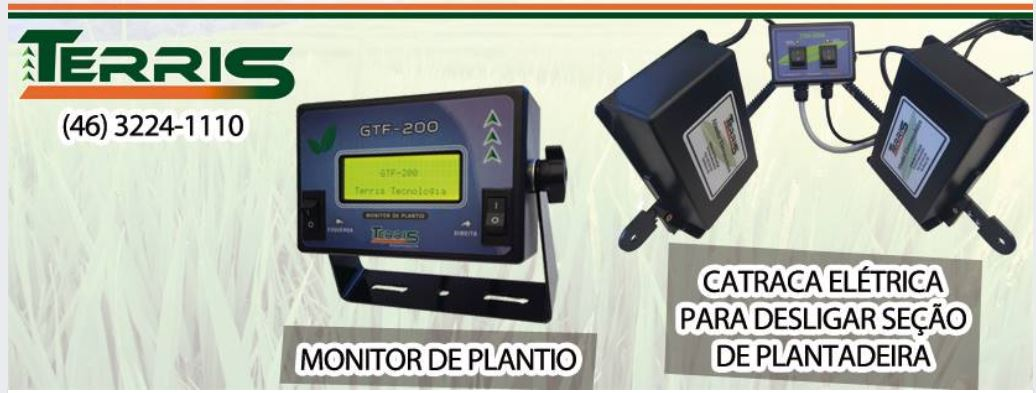
\includegraphics[width=\textwidth,keepaspectratio]{Figuras/Terris.jpg}
	 \caption{Logo da Terris}
	\end{figure}
	
	\column{0.4\linewidth}
	\begin{itemize}
	\item Terris automação agrícola
	\pause
	\item Empresa encubada
	\pause
	\item Produtos desenvolvidos e comercializados
	\end{itemize}

\end{columns}
\end{frame}

%%%%%%%%%%%%%%%%%%%%%%%%%%%%%%%%%%%%%%%%%%%%%%%%%%%%%%%%%%%%%%%%%%%%%%
\subsection{O Estágio}

\begin{frame}
\frametitle{O Estágio}

\begin{itemize}
	\item \textbf{Área de atuação}: Pesquisa e desenvolvimento
	\pause
	\item \textbf{Tipo de estágio}: Estudo dirigido
	\pause
	\item \textbf{Setor da empresa}: Pesquisa e desenvolvimento
	\pause	
	\item \textbf{Orientador(a)}: Professora Dra. Beatriz Terezinha Borsoi
	\pause
	\item \textbf{Contatos na empresa}: \\Sidney Gaspari\\ Josimar Tumeleiro
\end{itemize}
\end{frame}

%%%%%%%%%%%%%%%%%%%%%%%%%%%%%%%%%%%%%%%%%%%%%%%%%%%%%%%%%%%%%%%%%%%%%%%%%%%%%
\subsection{Atividade desenvolvida}
\begin{frame}
\frametitle{Atividade desenvolvida}

\begin{itemize}
	\item \textbf{Área de atuação}: Pesquisa e desenvolvimento
	\pause
	\item \textbf{Atividade}: Estudo dirigido
	\pause
	\item \textbf{Setor da empresa}: Pesquisa e desenvolvimento
	\pause	
	\item \textbf{Orientador(a)}: Professora Dra. Beatriz Terezinha Borsoi
	\pause
	\item \textbf{Contatos na empresa}: \\Sidney Gaspari\\ Josimar Tumeleiro
	\pause

\end{itemize}
\end{frame}













%\subsection{Referencial teórico} % A subsection can be created just before a set of slides with a common theme to further break down your presentation into chunks

%\begin{frame}
%\frametitle{Robótica}
%\begin{columns}
%	\column{0.35\linewidth}
%	\begin{itemize}
%	\item Industriais
%	\item Médicos
%	\item Móveis
%		\begin{itemize}
%		\item Com pernas (\textit{legged})
%		\item Com rodas (\textit{wheeled})
%		\end{itemize}
%	\end{itemize}
%
%	\column{0.7\linewidth}
%	 \begin{figure}[h]
%     \centering
%     \captionsetup{width=\textwidth,font=footnotesize,textfont=bf}
%     \begin{subfigure}[b]{0.5\textwidth}
% 	\centering
%         \includegraphics[width=\textwidth,height=\textheight,keepaspectratio]{Figuras/nasa.png}
%         \caption{\centering \label{fig:Testen}}
%     \end{subfigure}
%     
%     \begin{subfigure}[b]{0.5\textwidth}
% 	\centering
%         \includegraphics[width=\textwidth,height=5\textheight,keepaspectratio]{Figuras/Boston.png}
%         \caption{\centering \label{fig:Testeo}}
%     \end{subfigure}
%	\caption{Robôs móveis: (a) Robô Sojourner (NASA,1997);(b) \textit{Legged Squad Support System} (DYNAMICS,2016)}
% \end{figure}
%	
%\end{columns}
%\end{frame}




%%------------------------------------------------
%
%\begin{frame}
%\frametitle{Controle de tempo contínuo}
%\begin{columns}
%	\column{0.45\linewidth}
%	\begin{itemize}
%	\item Malha aberta
%	\item Malha fechada
%	\item Controlador
%		\begin{itemize}
%		\item Proporcional
%		\item Integral
%		\item Derivativa
%		\end{itemize}
%	\end{itemize}
%	
%	\column{0.6\linewidth}
%	\begin{figure}[h]
%     \centering
%     \captionsetup{width=\textwidth,font=footnotesize,textfont=bf}
%     \begin{subfigure}[b]{\textwidth}
% 	\centering
%         \includegraphics[width=\textwidth,height=\textheight,keepaspectratio]{Figuras/MalhaAberta.pdf}
%         \caption{\centering \label{fig:jkl}}
%     \end{subfigure}
%     
%     \begin{subfigure}[b]{\textwidth}
% 	\centering
%         \includegraphics[width=\textwidth,height=5\textheight,keepaspectratio]{Figuras/Controlador.pdf}
%         \caption{\centering \label{fig:ppolk}}
%     \end{subfigure}
%	\caption{Diagramas de controle: (a) Malha aberta;(b) Malha fechada com controlador}
% \end{figure}
%	
%\end{columns}
%\end{frame}
%
%%------------------------------------------------
%
%\begin{frame}
%\frametitle{Controle a eventos discretos}
%\begin{columns}
%	\column{0.3\linewidth}
%	\begin{itemize}
%	\item Eventos discretos
%	\item Autômato
%		\begin{itemize}
%		\item Moore
%		\item Mealy
%		\end{itemize}
%	\end{itemize}
%	
%	\column{0.7\linewidth}
%	\begin{figure}[h]
%     \centering
%     \captionsetup{width=0.85\textwidth,font=footnotesize,textfont=bf}
%     \begin{subfigure}[b]{\textwidth}
% 	\centering
%         \includegraphics[width=0.85\textwidth,height=\textheight,keepaspectratio]{Figuras/moore.pdf}
%         \caption{\centering \label{fig:moore}}
%     \end{subfigure}
%     
%     \begin{subfigure}[b]{\textwidth}
% 	\centering
%         \includegraphics[width=0.85\textwidth,height=5\textheight,keepaspectratio]{Figuras/mealy.pdf}
%         \caption{\centering \label{fig:mealy}}
%     \end{subfigure}
%	\caption{Autômatos: (a) Moore; (b) Mealy}
% \end{figure}
%	
%\end{columns}
%\end{frame}
%
%
%\begin{frame}
%\frametitle{Trabalho de Petry (2016)}
%\begin{columns}
%	\column{0.3\linewidth}
%	\begin{itemize}
%	\item Controle híbrido
%	\item Controlador PID
%	\item Lógica \textit{fuzzy}
%	\end{itemize}
%	
%	\column{0.7\linewidth}
%	\begin{figure}[h]
%     \centering
%     \captionsetup{width=0.9\textwidth,font=footnotesize,textfont=bf}
%     \begin{subfigure}[b]{0.4\textwidth}
% 	\centering
%         \includegraphics[width=1\textwidth,height=0.4\textheight]{Figuras/marcio1.png}
%         \caption{\centering \label{fig:marcio1}}
%     \end{subfigure}
%	~     
%     \begin{subfigure}[b]{0.4\textwidth}
% 	\centering
%         \includegraphics[width=1\textwidth,height=0.4\textheight]{Figuras/polulumod.png}
%         \caption{\centering \label{fig:pololumarcio}}
%     \end{subfigure}
%	\caption{Robôs de Petry (2016): (a) \textit{Alpha project}; (b) Pololu 3pi modificado}
% \end{figure}
%	
%\end{columns}
%\end{frame}

%------------------------------------------------

%\subsection{Cenário atual}
%
%
%
%\begin{frame}
%\frametitle{Cenário atual}
%%\%begin{columns}[c]
%
%	
%	\begin{itemize}
%	\item ART (\textit{ Autonomous Rail Rapid Transit} ou Trilho Autônomo de Trânsito 	Rápido)
%	\item Trem em Zhuzhou (China)
%	\end{itemize}
%
%	\begin{figure}[]
%	 \centering
%	 \captionsetup{width=0.7\textwidth,font=footnotesize,textfont=bf}
%	 \includegraphics[width=0.7\textwidth,keepaspectratio]{Figuras/Trem.jpg}
%	 \caption{Trem sobre trilhos virtuais}
%	\end{figure}
%
%%\end{columns}
%\end{frame}
%
%\subsection{Objetivos}
%
%\begin{frame}
%\frametitle{Objetivos}
%\begin{block}{Geral}
%	 Projetar e implementar um protótipo de um robô seguidor de linha, que seja autônomo, através da utilização de controle híbrido, aperfeiçoando as técnicas desenvolvidas por Petry (2016).
%\end{block}
%
%\begin{block}{Específicos}
%	\begin{itemize}
%	\item Projetar o condicionamento de sinais necessários para os dispositivos a serem utilizados, permitindo uma precisão na leitura dos sensores;
%	\item Projetar e confeccionar a estrutura do protótipo, visando atender as dimensões especificadas pela Robocore;
%	\item Implementar um controlador de Sistemas a Eventos Discretos, para que seja possível tratar de maneira precisa as marcações laterais da pista;
%
%	\end{itemize}
%\end{block}
%
%\end{frame}
%
%\begin{frame}
%\frametitle{Objetivos}
%\begin{block}{Específicos}
%	\begin{itemize}
%	\item Modelar a função de transferência do robô;
%	\item Implementar um controlador para manter o robô sobre a linha na pista;
%	\item Realizar testes com o protótipo em pistas que sigam as normas da Robocore;
%	\item Fazer o mapeamento do percurso com um \textit{encoder} para o controle da velocidade.
%	\item Comparar os resultados obtidos com o de Petry (2016).
%	\end{itemize}
%\end{block}
%
%\end{frame}

%------------------------------------------------

%\begin{frame}
%\frametitle{Multiple Columns}
%\begin{columns}[c] % The "c" option specifies centered vertical alignment while the "t" option is used for top vertical alignment
%
%\column{.45\textwidth} % Left column and width
%\textbf{Heading}
%\begin{enumerate}
%\item Statement
%\item Explanation
%\item Example
%\end{enumerate}
%
%\column{.5\textwidth} % Right column and width
%Lorem ipsum dolor sit amet, consectetur adipiscing elit. Integer lectus nisl, ultricies in feugiat rutrum, porttitor sit amet augue. Aliquam ut tortor mauris. Sed volutpat ante purus, quis accumsan dolor.
%
%\end{columns}
%\end{frame}

%------------------------------------------------


%%------------------------------------------------
%\section{Justificativa}
%
%
%
%\begin{frame}
%\frametitle{Justificativa}
%\begin{columns}[c]
%
%	\column{0.4\textwidth}
%	\begin{figure}[h]
%     \centering
%     \captionsetup{width=0.85\textwidth,font=footnotesize,textfont=bf}
%     \begin{subfigure}[b]{\textwidth}
% 	\centering
%         \includegraphics[width=0.85\textwidth,height=\textheight,keepaspectratio]{Figuras/robogames.jpg}
%         \caption{\centering \label{fig:fss}}
%     \end{subfigure}
%     
%     \begin{subfigure}[b]{\textwidth}
% 	\centering
%         \includegraphics[width=0.85\textwidth,height=5\textheight,keepaspectratio]{Figuras/winterlogo.jpg}
%         \caption{\centering \label{fig:vdd}}
%     \end{subfigure}
%	\caption{Competições: (a) Robogames; (b) WinterChallenge}
% \end{figure}
%	\pause
%	\column{0.6\textwidth}
%	\begin{itemize}
%	\item ART (\textit{ Autonomous Rail Rapid Transit} ou Trilho Autônomo de Trânsito 	Rápido)
%	\item Trem em Zhuzhou (China)
%	\end{itemize}
%
%	\begin{figure}[]
%	 \centering
%	 \captionsetup{width=0.7\textwidth,font=footnotesize,textfont=bf}
%	 \includegraphics[width=0.7\textwidth,keepaspectratio]{Figuras/Trem.jpg}
%	 \caption{Trem sobre trilhos virtuais (DAILYMAIL, 2017)}
%	\end{figure}
%
%\end{columns}
%\end{frame}


%%%%%%%%%%%%%%%%%%%%%%% EOF %%%%%%%%%%%%%%%%%%%%%%%%%%%%
%%\input{Objetivos}
%
\section{Materiais}

%% Tentar fazer a transição deste slide
%\begin{frame}
%\begin{figure}[]
%	\frametitle{Materiais}
%     \centering
%     \captionsetup{width=\textwidth,font=footnotesize,textfont=bf}   
%     \begin{subfigure}[b]{0.2\textwidth}
% 	\centering
%         \includegraphics[width=\textwidth,height=\textheight,keepaspectratio]{Figuras/motor.png}
%         \caption{\centering \label{fig:Posicaofinal}}
%     \end{subfigure}
%     \caption{Materiais utilizados}
%    
% \end{figure}
%\end{frame}


\begin{frame}
\vspace{-0.4cm}
\begin{figure}[noframenumbering]
	\frametitle{Materiais}
     \centering
     \captionsetup{width=\textwidth,font=footnotesize,textfont=bf}
     \begin{subfigure}[b]{0.2\textwidth}
 	\centering
         \includegraphics[width=\textwidth,height=\textheight,keepaspectratio]{Figuras/motor.png}
         \caption{\centering \label{fig:a1}}
     \end{subfigure}
     ~
     \begin{subfigure}[b]{0.2\textwidth}
 	\centering
         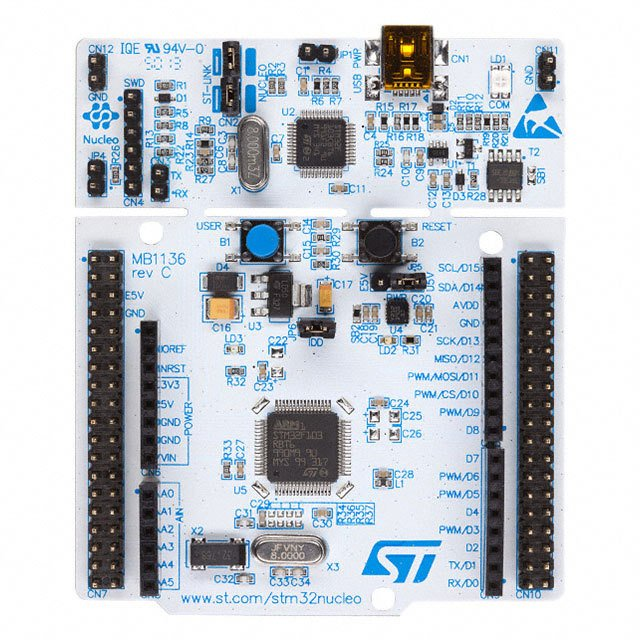
\includegraphics[width=\textwidth,height=0.3\textheight,keepaspectratio]{Figuras/nucleo.jpg}
         \caption{\centering \label{fig:a2}}
     \end{subfigure}
     ~
     \begin{subfigure}[b]{0.2\textwidth}
 	\centering
         \includegraphics[width=\textwidth,height=0.3\textheight,keepaspectratio]{Figuras/sparkfun.jpg}
         \caption{\centering \label{fig:a3}}
     \end{subfigure}
          ~
     \begin{subfigure}[b]{0.2\textwidth}
 	\centering
         \includegraphics[width=\textwidth,height=0.4\textheight,keepaspectratio]{Figuras/encoder.png}
         \caption{\centering \label{fig:a4}}
     \end{subfigure}
     
     \begin{subfigure}[b]{0.2\textwidth}
 	\centering
         \includegraphics[width=\textwidth,height=1.2\textheight,keepaspectratio]{Figuras/stepup.jpg}
         \caption{\centering \label{fig:b1}}
     \end{subfigure}
     ~
     \begin{subfigure}[b]{0.2\textwidth}
 	\centering
         \includegraphics[width=\textwidth,height=0.3\textheight,keepaspectratio]{Figuras/Lipo.png}
         \caption{\centering \label{fig:b2}}
     \end{subfigure}
     ~
     \begin{subfigure}[b]{0.2\textwidth}
 	\centering
         \includegraphics[width=0.7\textwidth,height=0.3\textheight,keepaspectratio]{Figuras/hc05.png}
         \caption{\centering \label{fig:b3}}
     \end{subfigure}
          ~
     \begin{subfigure}[b]{0.2\textwidth}
 	\centering
         \includegraphics[width=\textwidth,height=0.3\textheight,keepaspectratio]{Figuras/qre.jpg}
         \caption{\centering \label{fig:b4}}
     \end{subfigure}
     
     \caption{Materiais utilizados: (a) Motor Pololu; (b) Nucleo-STM32F303K8; (c) TB6612FNG; (d) \textit{Encoder} Pololu; (e) \textit{Step up}; (f) Bateria LiPo; (g) HC05; (h) QRE1113}     
 \end{figure}
\end{frame}

\begin{frame}
\frametitle{Softwares utilizados}

\begin{itemize}
\item Inkscape;
\item Matlab;
\item Kicad;
\item Supremica;
\item Deslab;
\item STM32 CubeMX;
\item System Workbench;
\item Linguagem C;
\item \LaTeX

\end{itemize}
\end{frame}


%\input{Metodologia.tex}
%\input{Implementacao.tex}
%------------------------------------------------
\section{Desenvolvimento e resultados}
%------------------------------------------------

%%%%%%%%%%%%%%%%%%%%%%%%%%%%%%%%%%%%%%%%%%%%%%%%%%%%%%%%%%%
%%%%%%%%%%%%%%%%%%%%%%%%%%%%%%%%%%%%%%%%%%%%%%%%%%%%%%%%%%%

\subsection{O Projeto}

\begin{frame}
\frametitle{O Projeto}
\begin{enumerate}
\item Estudo da tecnologia;
\pause \item Comparativo entre os módulos;
\pause \item Implementação no microcontrolador.
\end{enumerate}
\end{frame}

\subsection{Estudo da tecnologia}

\begin{frame}
\frametitle{Estudo da tecnologia}
\begin{itemize}
\item Estudo do NMEA;
\pause
\item Estudo dos módulos de GPS da u-blocks:
	\begin{itemize}
	\item NEO-6M;
	\item LEA-6H;
	\end{itemize}
\pause
\item IDE Coocox e bibliotecas CMSIS;
\end{itemize}
\end{frame}

\subsection{Comparativo entre os módulos}

\begin{frame}
\frametitle{Comparativo entre os módulos}
\begin{columns}

	\column{0.4\linewidth}
	\begin{itemize}
	\item Comparação feita com o Arduino;
	\item Informações salvas em um cartão SD;
	\item Testes definitivos feitos na pista de atletismo da UTFPR;
	\item Informações graficadas no \textit{software} Google Earth;
	\item Desenvolvimento de uma \textit{shield} para o Arduino Mega;
	\end{itemize}

	\column{0.7\linewidth}
	\begin{figure}[]
	 \centering
	 \captionsetup{width=0.9\textwidth,font=footnotesize,textfont=bf}
	 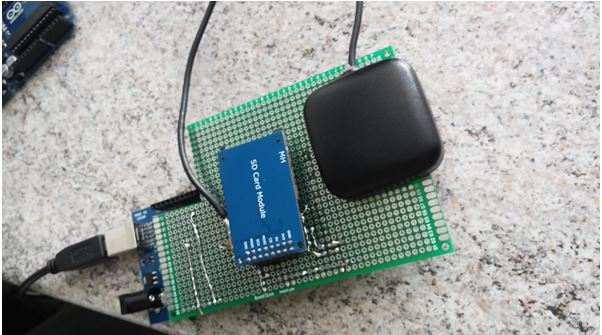
\includegraphics[width=0.9\textwidth,keepaspectratio]{Figuras/shield.jpg}
	 \caption{Shield para o Arduino}
	\end{figure}
	
\end{columns}
\end{frame}




\begin{frame}
\frametitle{Comparativo entre os módulos}

	\begin{figure}[]
	 \centering
	 \captionsetup{width=0.9\textwidth,font=footnotesize,textfont=bf}
	 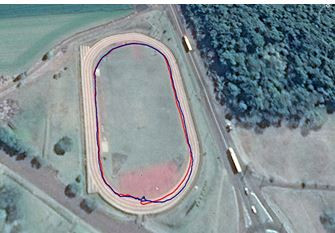
\includegraphics[width=0.9\textwidth,keepaspectratio]{Figuras/teste.jpg}
	 \caption{Comparativo entre os dois módulos (Vermelho: LEA-6H; Azul: NEO-6M)}
	\end{figure}
\end{frame}



\begin{frame}
\frametitle{Comparativo entre os módulos}
	
	\begin{figure}[]
	 \centering
	 \captionsetup{width=\textwidth,font=footnotesize,textfont=bf}
	 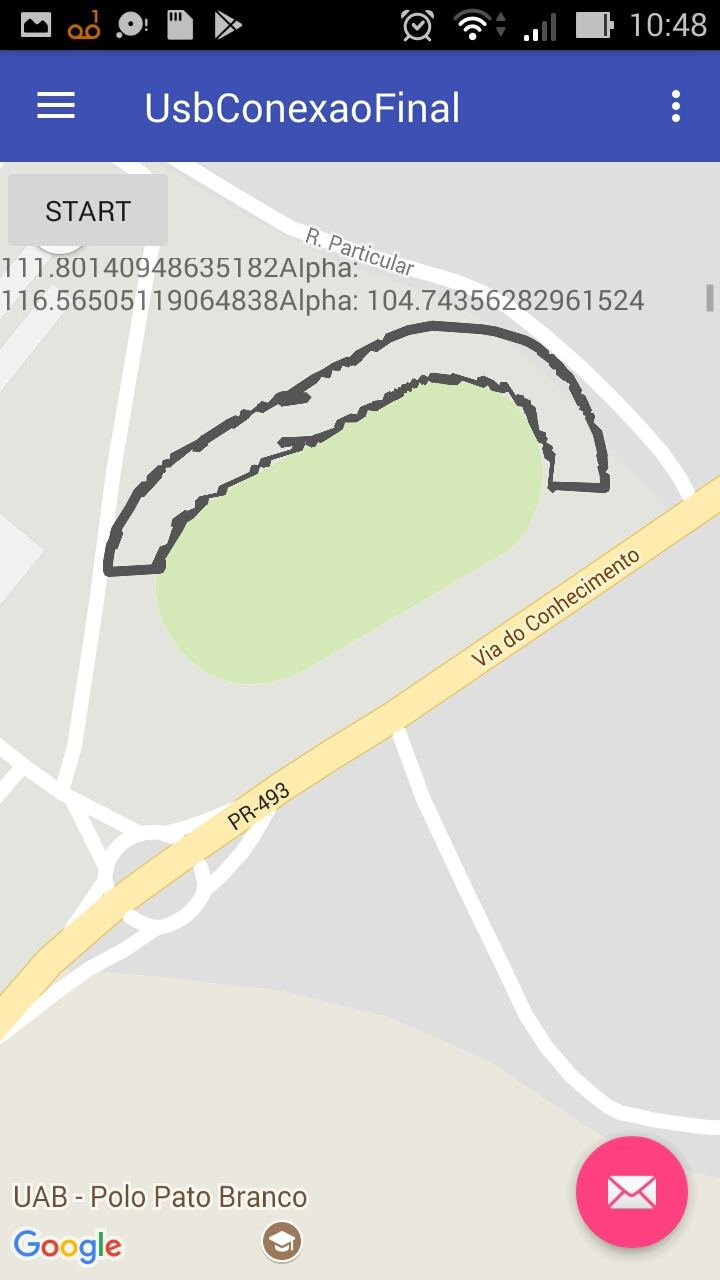
\includegraphics[width=0.5\textwidth,height=0.75\textheight,keepaspectratio]{Figuras/integracao.jpg}
	 \caption{Integração dos trabalhos desenvolvidos na Terris (Hamilton, Vinícius e Willian)}
	\end{figure}
	
\end{frame}




%%%%%%%%%%%%%%%%%%%%%%%%%%%%%%%%%%%%%%%%%%%%%%%%%%%%%%%%%%%%%%%%
\subsection{Implementação no microcontrolador}

\begin{frame}
\frametitle{Implementação no microcontrolador}
\begin{columns}

	\column{0.4\linewidth}
	\begin{itemize}
	\item Dados obtidos pela sentença GPRMC;
	\item Informações obtidas: longitude, latitude, velocidade de deslocamento e tempo de aquisição do sinal;
	\end{itemize}

	\column{0.7\linewidth}
	\begin{figure}[]
	 \centering
	 \captionsetup{width=0.9\textwidth,font=footnotesize,textfont=bf}
	 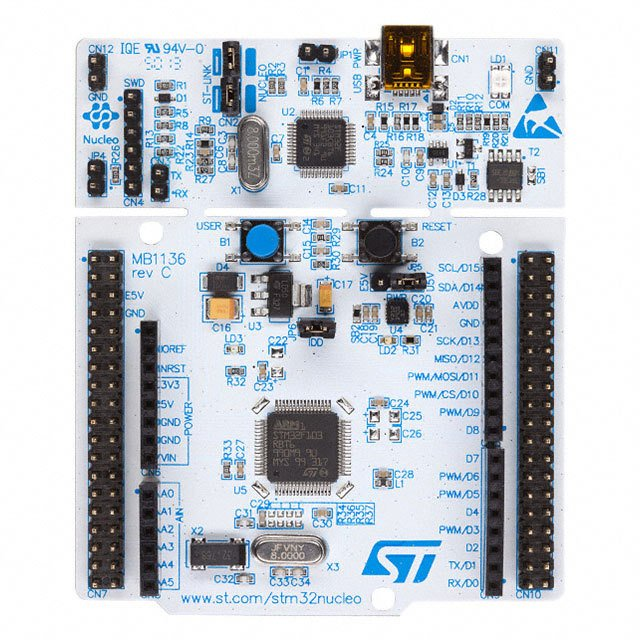
\includegraphics[width=0.9\textwidth,keepaspectratio]{Figuras/nucleo.jpg}
	 \vspace{-0.2cm}
	 \caption{Microcontrolador utilizado}
	\end{figure}
	
\end{columns}
\end{frame}

%%%%%%%%%%%%%%%%%%%%% EOF %%%%%%%%%%%%%%%%%%%%%%%
%%------------------------------------------------
\section{Oportunidades de desenvolvimento}
%------------------------------------------------

%%%%%%%%%%%%%%%%%%%%%%%%%%%%%%%%%%%%%%%%%%%%%%%%%%%%%%%%%%%
%%%%%%%%%%%%%%%%%%%%%%%%%%%%%%%%%%%%%%%%%%%%%%%%%%%%%%%%%%%

\begin{frame}
\frametitle{Oportunidades de desenvolvimento}
\begin{itemize}
\item Fácil adaptação à empresa;
\item Novos conhecimento aprendidos;
\item Cotidiano de uma empresa;
\item Área com grande potencial.
\end{itemize}
\end{frame}

%------------------------------------------------
\section{Dificuldades encontradas}
%------------------------------------------------

%%%%%%%%%%%%%%%%%%%%%%%%%%%%%%%%%%%%%%%%%%%%%%%%%%%%%%%%%%%
%%%%%%%%%%%%%%%%%%%%%%%%%%%%%%%%%%%%%%%%%%%%%%%%%%%%%%%%%%%

\begin{frame}
\frametitle{Dificuldades encontradas}
\begin{itemize}
\item Horário escasso dos supervisores na Terris;
\item Microcontrolador (IDE e bibliotecas).
\end{itemize}
\end{frame}


%------------------------------------------------
\section{Conclusão e sugestões}
%------------------------------------------------

%%%%%%%%%%%%%%%%%%%%%%%%%%%%%%%%%%%%%%%%%%%%%%%%%%%%%%%%%%%
%%%%%%%%%%%%%%%%%%%%%%%%%%%%%%%%%%%%%%%%%%%%%%%%%%%%%%%%%%%

\begin{frame}
\frametitle{Conclusão e sugestões}

\begin{block}{Conclusão}
\begin{itemize}
\item Atividades finalizadas;
\item LEA-6H com melhor desempenho;
\item Necessária a melhoria deste sinal (precisão);
\end{itemize}
\end{block}

\begin{block}{Sugestões}
\begin{itemize}
\item Adoção de cronograma de trabalho;
\item Ferramenta de desenvolvimento de \textit{software} conjunto (Github);
\item Implementação de filtros no sinal do GPS
\end{itemize}
\end{block}

\end{frame}

%%%%%%%%%%%%%%%%%%%% EOF %%%%%%%%%%%%%%%%
%\input{Referencias.tex}
%------------------------------------------------

%% Repeat the title page
\againframe{firstframe}


%----------------------------------------------------------------------------------------

\end{document} 